\chapter{Implementation Results}

% You can title this chapter as \textbf{Preliminary Results} or \textbf{Work Progress} for the progress reports. Present implementation or experimental results here and discuss them.


% ALL SECTIONS IN THIS CHAPTER ARE OPTIONAL. PLEASE CONSULT YOU ADVISOR AND DESIGN YOUR OWN SECTION

% \emph{\textthai{หัวข้อต่าง ๆ ในแต่ละบทเป็นเพียงตัวอย่างเท่านั้น หัวข้อที่จะใส่ในแต่ละบทขึ้นอยู่กับโปรเจคของนักศึกษาและอาจารย์ที่ปรึกษา}}
\section{Introduction}
This chapter provides a comprehensive overview of the results derived from all the implementations undertaken throughout the project. It elaborates on the methodologies employed for testing, including a detailed explanation of the processes and techniques used to ensure accuracy and reliability. Additionally, it specifies the sources of information utilized, highlighting their relevance and credibility in supporting the project objectives. Furthermore, the chapter outlines the evaluation criteria applied to each test, offering a clear framework for assessing the effectiveness and success of the implemented solutions. This structured approach ensures transparency and provides a solid foundation for interpreting the outcomes of the project.

\section{Phase 1}
    \subsection{Prompt Tuning}
    To evaluate the overall performance of the Query Assistance prompt, prompt tuning is conducted. This approach is prioritized due to the agent's heavy reliance on prompts. Ensuring the effectiveness of the prompt is critical, as it guides the agent to operate in alignment with its intended purpose.

    A comprehensive list of scenarios has been tested to assess the system's performance. For each scenario, corresponding test cases are developed and categorized into three levels of difficulty: easy, medium, and hard. For smaller scenarios, a reduced number of test cases is included. Additionally, the weight of these smaller scenarios in the overall performance evaluation is halved relative to the number of cases. The success rate for each scenario is then analyzed to provide insights into the system's effectiveness. Four versions of the prompt have been developed to optimize the performance of the Query Assistance system.
    \begin{itemize}
        \item The first version outlines general requirements for the Query Assistance system, including tasks such as adjusting queries to align with the specified database, adding limits, and other foundational functionalities.
        \item The second version was refined based on extensive testing across various cases. Observations revealed that the system handled subqueries poorly. To address this, the prompt was updated to emphasize handling subqueries effectively and managing specific scenarios, such as cases where no data is returned.
        \item The third version focuses on improving clarity and usability by reorganizing the prompt into distinct sections. This structural adjustment aims to facilitate the agent's ability to process and execute tasks more efficiently.
        \item The fourth version introduces a structured output format to enhance consistency and readability. Additionally, it emphasizes the importance of preserving correct table and column names, ensuring that these elements remain unaltered during query adjustments.
        \item The fifth version was developed after deploying the system for user access and making adjustments based on the results obtained and the analysis of error causes. The first issue we identified was its inability to properly handle arrays. Additionally, we observed that it did not consistently include basic optimizations, such as adding the partition column. To address these issues, we incorporated them into the prompt, which subsequently improved overall performance.
    \end{itemize}
    \begin{table}[H]
        \centering
        \caption[Result of Prompt Tuning]{Result of Prompt Tuning}
        \label{fig:prompt-tuning}
        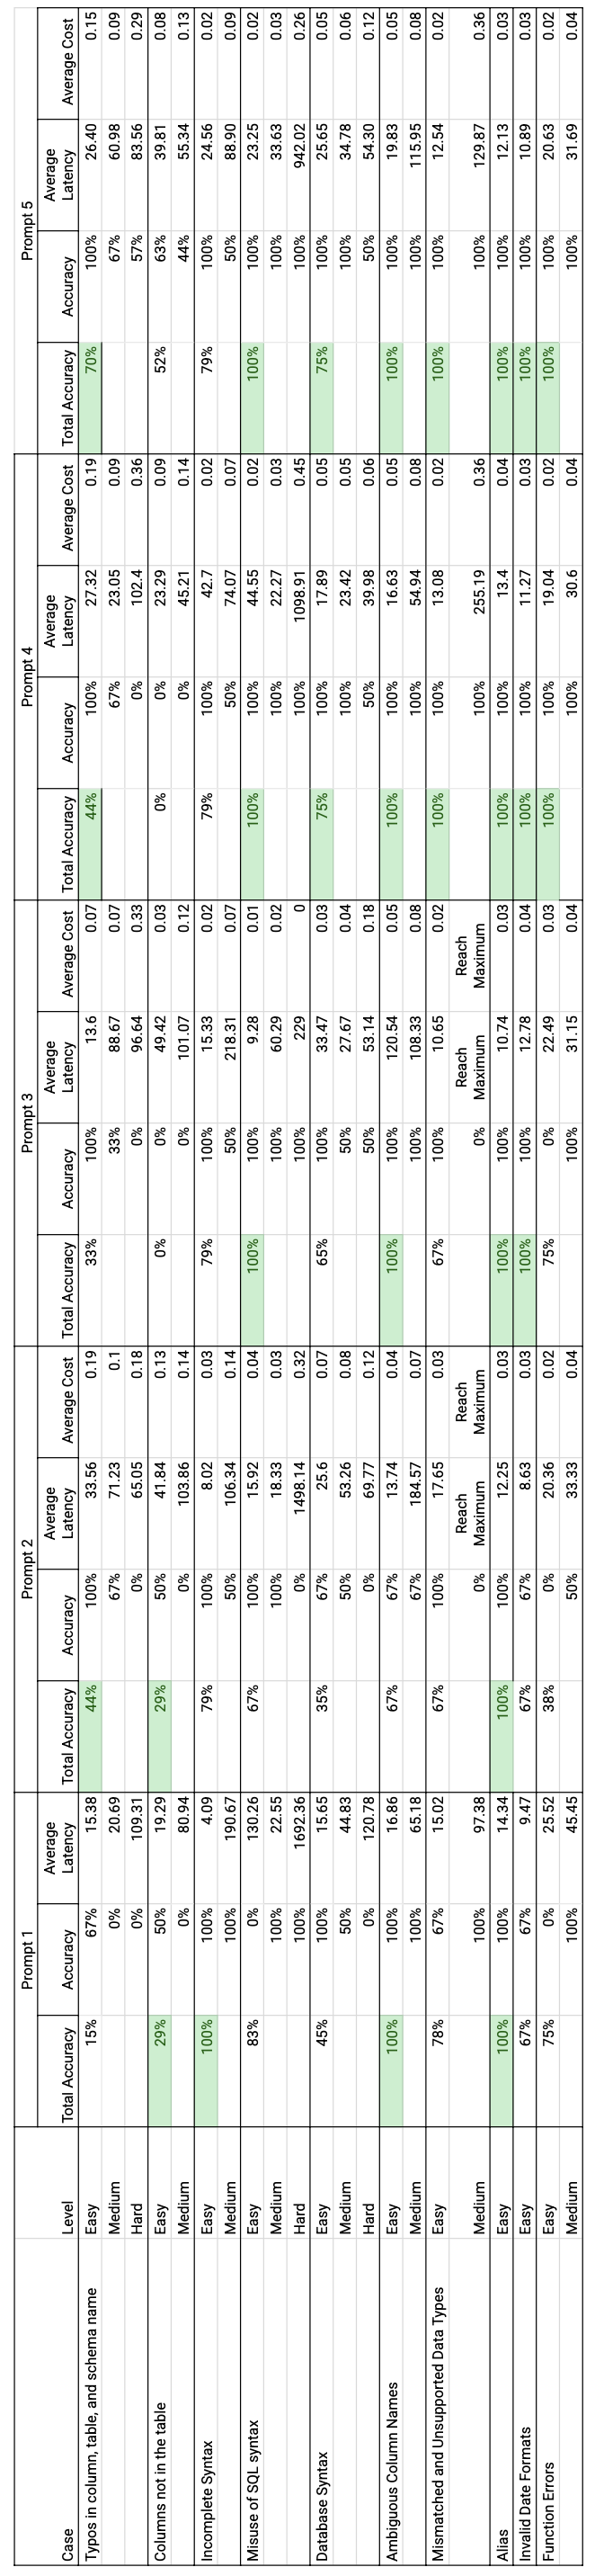
\includegraphics[width=6cm]{chapters/4/figures/prompt.png}
    \end{table}
    \textbf{Metrics for Evaluating}
    \begin{itemize}
        \item Latency is defined as the duration between the initiation of an API request and the receipt of the corresponding response. This metric is critical for evaluating the performance and responsiveness of the system, as it directly impacts user experience and operational efficiency. A lower latency indicates a faster and more efficient system, which is often a key objective in optimizing API interactions.
        \item Cost is determined using the get\_openai\_callback function provided by the LangChain Community (langchain\_community.callbacks). This function calculates the token usage and associated cost based on the specific OpenAI model employed. By leveraging this tool, we can accurately monitor and manage the financial implications of utilizing different models, ensuring cost-effectiveness while maintaining the desired level of performance and accuracy.
        \item Accuracy is assessed by analyzing the similarity and correctness of the SQL query results. This involves comparing the output against expected results to ensure they are aligned and capable of resolving the identified issue. A high level of accuracy is essential for maintaining the reliability and effectiveness of the system, as it ensures that the generated solutions are both relevant and actionable. This metric serves as a key indicator of the system's ability to address complex problems and deliver meaningful outcomes.
    \end{itemize}
\pagebreak

\section{Phase 2}
    \subsection{Model Evaluation}
    During the development of the Phase 2 query generation model, a series of evaluations was conducted to assess the performance of various models. The evaluation process involved testing multiple models with different tools. The primary objective was to identify the most effective model for generating SQL queries from natural language input. Models were evaluated both with and without Prefilter (a Workspace model), and cost was also considered as a decision factor.

    All tests were conducted using MLflow to record the testing procedures, results, and evaluations performed with OpenAI through MLflow. Since custom evaluation metrics could be defined, the following metrics were used to assess model performance:

    \begin{itemize}
        \item Table correction is defined as the degree to which the table name included in the output matches the ground truth table. This metric is essential for assessing the accuracy and relevance of the generated responses, as it ensures that the correct data source is referenced. A higher table correction score indicates that the output consistently includes the appropriate table, which is crucial for reliable query generation and data retrieval.
        \item Column correction is defined as the extent to which the column names present in the output align with those in the ground truth. This metric is crucial for evaluating the precision and reliability of generated responses, as it ensures that the correct columns are referenced in the answer. A higher column correction score reflects a more accurate and faithful representation of the intended data, which is essential for effective query generation
        \item Workspace correction is defined as the degree to which the workspace mentioned in the output matches the workspace specified in the ground truth. This metric is important for assessing the accuracy and relevance of the generated response, as it ensures that the correct workspace context is referenced. A higher workspace correction score indicates that the output consistently includes the appropriate workspace, which is essential for precise data categorization and retrieval.
        \item Description correction is defined as the extent to which the output description or the ground truth description better addresses the input question. This metric is essential for evaluating the relevance and quality of the provided descriptions, ensuring that the most appropriate and informative response is selected. A higher description correction score indicates that the output description is as suitable as, or more suitable than, the ground truth in answering the user's question, thereby enhancing the overall effectiveness and clarity of the response.
        \item Table usage metric is defined as the assessment of how well the table in the output, compared to the ground truth, is suited to address the input question based solely on its intended use. This metric focuses exclusively on the relevance and appropriateness of the table’s usage, disregarding other factors such as table name or description. A higher table usage score indicates that the selected table is more effective or equally effective in meeting the informational needs of the question, thereby supporting more accurate and contextually appropriate query generation.
    \end{itemize}

    The same prompt was used throughout the evaluation to ensure consistency and reliability in the process. All models had access to the basic tools: 'Retrieve table info' and 'Column validation'. For models utilizing Prefilter, the 'Retrieve table in workspace' tool was also included. For models without Prefilter, all available tables from our testing database were provided instead.
    \begin{itemize}
        \item Prefilter
        \begin{itemize}
            \item Model with Chart Summary tool
            \item Model with Pick table tool
            \item Model with Pick table and Chart Summary tool
        \end{itemize}
        \item Without Prefilter
        \begin{itemize}
            \item Model with Chart Summary tool
            \item Model with Pick table tool
            \item Model with Pick table and Chart Summary tool
        \end{itemize}
    \end{itemize}
    \begin{table}[H]
        \centering
        \caption[Result of Model Evaluation]{Result of Model Evaluation}
        \label{fig:generate_result}
        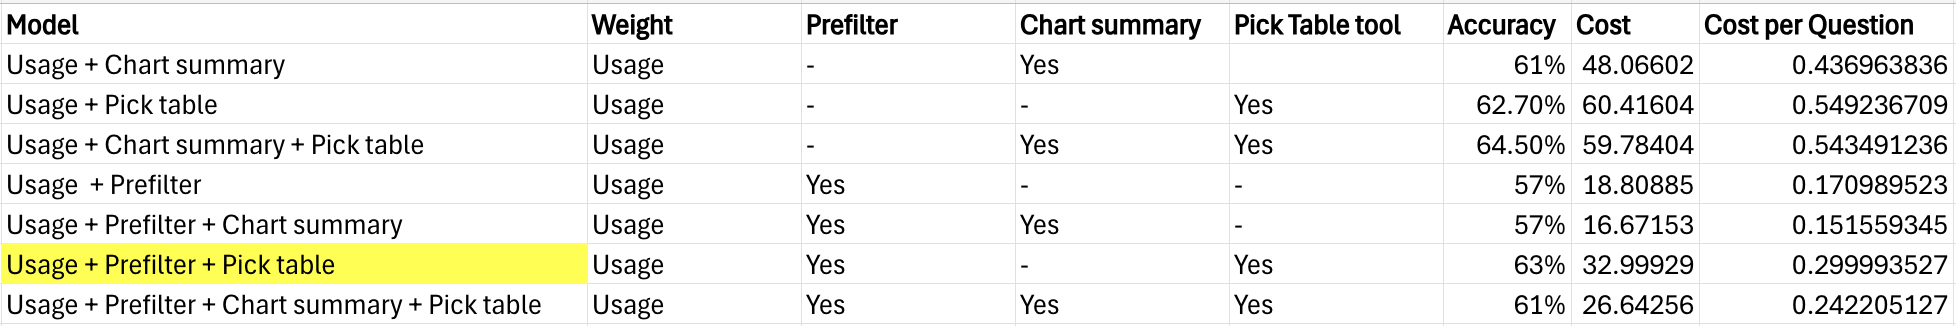
\includegraphics[width=17cm]{chapters/4/figures/generate_result.png}
    \end{table}
    According to the results chart, the highest accuracy achieved was 64.5\% with the Usage + Chart Summary + Pick Table model. However, when we compare the cost of this model to our latest model, Usage + Prefilter + Pick Table, we find that the cost nearly doubles for only a 1.5\% increase in accuracy. Therefore, we believe it is more practical to deploy the Usage + Prefilter + Pick Table model to production.
    \vspace{0.5cm}


    \textbf{Metrics for Evaluating}


    Although there are plenty of metrics to evaluate the model, we only focus on the following metrics in making the decision:
    \begin{itemize}
        \item Table correction is defined as the degree to which the table name included in the output matches the ground truth table. This metric is essential for assessing the accuracy and relevance of the generated responses, as it ensures that the correct data source is referenced. A higher table correction score indicates that the output consistently includes the appropriate table, which is crucial for reliable query generation and data retrieval.
        \item Column correction is defined as the extent to which the column names present in the output align with those in the ground truth. This metric is crucial for evaluating the precision and reliability of generated responses, as it ensures that the correct columns are referenced in the answer. A higher column correction score reflects a more accurate and faithful representation of the intended data, which is essential for effective query generation and data analysis.
        \item Cost is determined using the get\_openai\_callback function provided by the LangChain Community (langchain\_community.callbacks). This function calculates the token usage and associated cost based on the specific OpenAI model employed. By leveraging this tool, we can accurately monitor and manage the financial implications of utilizing different models, ensuring cost-effectiveness while maintaining the desired level of performance and accuracy.
    \end{itemize}

\section{Phase 3}
    In this phase, testing is conducted using a straightforward approach to evaluate the readiness of the general question agent.
    \begin{table}[H]
      \centering
      \caption{General Agent Testing Result}
      \label{tbl:general-agent-testing-result}
      \begin{tabular}{|l|c|c|c|}
        \hline
        \textbf{Testing Type} & \textbf{Score} & \textbf{Count} & \textbf{Percentage} \\
        \hline
        \multirow{4}{*}{General Question}
                  & 4 & 1 & 10\% \\
                  & 3 & 1 & 10\% \\
                  & 2 & 7 & 70\% \\
                  & 1 & 1 & 10\% \\
        \hline
        \multirow{4}{*}{Comparison Question}
                  & 4 & 8 & 80\% \\
                  & 3 & 1 & 10\% \\
                  & 2 & 1 & 10\% \\
                  & 1 & 0 & 0\% \\
        \hline
      \end{tabular}
    \end{table}
    \textbf{Metrics for Evaluating}
    \begin{itemize}
      \item Data Description correctness: \\ This metric evaluates whether the LLM’s (Large Language Model’s) result aligns with the ground truth. A higher score indicates greater accuracy and relevance. The scoring system is as follows:
      \begin{itemize}
        \item 4: The LLM's response is more accurate than the ground truth.
        \item 3: The result exactly matches the ground truth.
        \item 2: The result is partially related to the ground truth.
        \item 1: The result is not related to the ground truth at all.
      \end{itemize}
    \end{itemize}
